\section[Análisis Financiero]{Análisis Financiero}

\subsection{Análisis financiero del hardware}
En el proyecto se analizaron los gastos teniendo en cuenta  recursos materiales y humanos utilizados. 
Para el calcular el proceso de esfuerzo humano se realizó un promedio del salario en base a un desarrollador de software en Paraguay. 
Como el proyecto está hecho con lenguajes de programación web para el software y lenguaje C para el hardware se vio que los Desarrolladores web y multimedia ganan normalmente un salario neto mensual aproximado de entre Gs. 3.000.000 y Gs. 6.000.000 al empezar en el puesto de trabajo, esto según las referencias obtenidas de la página tusalario.org,~\cite{tusalario}, así haciendo un promedio y suponiendo 20 días de trabajo al mes con 8 horas diarias, el costo por horas de trabajo es de 30 000Gs por hora aproximadamente. 
Se aborda este salario para el trabajo en \textit{backend}, \textit{frontend}, desarrollo de hardware y su programación. 
Como no se trabaja las 8 horas diarias por el desarrollo del sistema, empleamos 4 horas diarias para el desarrollo y las restantes 4 horas para otras gestiones e investigaciones que no carga con las horas del diseño en sí. 

En la Tabla~\ref{tabla:hw} se observa el costo de los componentes utilizados para el hardware, además de las herramientas utilizadas para su elaboración. 


%%%%%%%%%%%%%%%%%%%%% tabla %%%%%%%%%%%%%%%%%%%%%%%%%%%%%%%%
\begin{table}[H]
\begin{center}
\begin{tabular}{c l l r r }
\toprule
\textbf{Cant} & \textbf{Componente} & \textbf{Descripción} &\textbf{Unidad Gs.}&\textbf{Importe Gs.}  \\ 
\midrule
2    & Capacitores      & 10uF        & 250            & 500   \\ 
%\hline
2    & Capacitores      & 0,1uF       & 250            & 500   \\ 
%\hline
2    & Capacitores      & 15pf        & 1.000           & 2.000  \\ 
%\hline
1    & Resistor         & 330 ohm     & 250            & 250   \\ 
%\hline
1    & Resistor         & 100k        & 250            & 250   \\ 
%\hline
1    & Microcontrolador &PIC18F4580   & 85.000          & 85.000 \\ 
%\hline
1    & Regulador        & 7805        & 15.000          & 15.000 \\ 
%\hline
2    & Diodo            & 1N4148      & 1.000           & 2.000  \\ 
%\hline
1    & Diodo Led        & Rojo        & 1.000           & 1.000  \\ 
%\hline
1    & Botón            & 4 pines    & 3.500           & 3.500  \\ 
%\hline
1    & Conector        & DB9    & 5.000           & 5.000  \\ 
%\hline
1    & Espadines       & 5 pines   & 3.500           & 3500  \\ 
%\hline
2    & Módulo          & SHIELD & 55.000          & 110.000 \\ 
%\hline
2    & Módulo          & XBEE        & 250.000         & 500.000 \\ 
%\hline
2    & Espadines       & 20 pines  & 3.500           & 7.000    \\ 
%\hline
1    & Módulo          & MCP2551     & 30.000          & 30.000  \\ 
%\hline
1    & Cristal         & 16Mhz     & 5.000           & 5.000   \\ 
%\hline
1    & Placa de Cobre  & 1 Capa      & 13.000          & 13.000   \\ 
%\hline
1    & Conector OBD II  & OBD II     & 50.000          & 50.000   \\ 
%\hline
1    & Impresora 3D         & Caja 3D       & 100.000         & 100.000 \\ 
%\hline
1    & Fresadora CNC    & CNC        & 100.000         & 100.000 \\ 
%\hline
      &                  &            & \textbf{Total} & \textbf{1.033.500}  \\ 
      \bottomrule
\end{tabular}
\caption{Costo de los componentes y herramientas usadas en el hardware.}
\label{tabla:hw}
\end{center}
\end{table}

Para la programación  y diseño organizaremos el trabajo en diseño del hardware, programación del hardware, Programación del Software \textit{frontend} y \textit{backend}, cada uno con un costo de 30.000Gs. la hora, resultando lo visto en la Tabla~\ref{tabla:software}. 

%%%%%%%%%%%%%%%%%%%%% tabla %%%%%%%%%%%%%%%%%%%%%%%%%%%%%%%%
\begin{table}[H]
\begin{center}
\begin{tabular}{l r r r}
\toprule
\textbf{Trabajo Realizado} & \textbf{Horas}&\textbf{Salario por hora Gs.} & \textbf{Importe Gs.} \\ \hline

 Placa Electrónica & 160 & 30.000  & 4.800.000     \\ 
 %\hline
 Software CAN      & 320 & 30.000  & 9.600.000     \\ 
 %\hline
 Diseño de Usuario & 320 & 30.000  & 9.600,000     \\ 
 %\hline
 Programación del Servidor & 320 & 30.000 & 9.600.000 \\ 
 %\hline 
 \textbf{ Total Costos} &  & & 33.600.000 \\ %\hline 
\bottomrule
\end{tabular}
\caption{Tabla Costos de mano de obra.}
\label{tabla:software}
\end{center}
\end{table}
%%%%%%%%%%%%%%%%%%%%%%%%%%%%%%%%%%%%%%%%%%%%%%%%%%%%%%%%%%%%%%%%%%%%



En la Tabla \ref{tabla:licencias} observamos el costo de las licencias de Proteus~\cite{licenp}, y el compilador PIC CCS~\cite{pic_ccs}.
%%%%%%%%%%%%%%%%%%%%% tabla %%%%%%%%%%%%%%%%%%%%%%%%%%%%%%%%
%%%% \textbf{tabla \ref{tabla:hw}} 
\begin{table}[H]
\begin{center}
\begin{tabular}{l l r }
\toprule
\textbf{Herramienta} & \textbf{Licencia} & \textbf{Costo}  \\ 
\midrule
Proteus Starter Kit  & Básica & 1.600.000  \\ 
Compilador PIC CCS   & PIC18  & 1.400.000  \\ 
\textbf{Total Costos} &  &   3.000.000     \\ \bottomrule
\end{tabular}
\caption{Tabla Costos de Licencias.}
\label{tabla:licencias}
\end{center}
\end{table}
%%%%%%%%%%%%%%%%%%%%%%%%%%%%%%%%%%%%%%%%%%%%%%%%%%%%%%%%%%%%%%%%


En la Tabla \ref{tabla:total} presentamos el costo total del proyecto teniendo en cuenta los resultados de las tablas anteriores: 

%%%%%%%%%%%%%%%%%%%%% tabla %%%%%%%%%%%%%%%%%%%%%%%%%%%%%%%%
%%%% \textbf{tabla \ref{tabla:hw}} 
\begin{table}[H]
\begin{center}
\begin{tabular}{l r}
\toprule
\textbf{Referencia} & \textbf{Costos}  \\ 
\midrule
Costos Hardware  & 1.033.500\\ 
%\hline
Costos Mano de Obra  & 33.600.000     \\ 
%\hline
Costos Licencias & 3.000.000\\ 
%\hline
\textbf{Total Costos} & 37.633.500    \\ 
%\hline
\bottomrule
\end{tabular}
\caption{Tabla costos totales.}
\label{tabla:total}
\end{center}
\end{table}
%%%%%%%%%%%%%%%%%%%%%%%%%%%%%%%%%%%%%%%%%%%%%%%%%%%%%%%%%%%%%%%%

Así el costo mínimo del proyecto sería de 37.633.500 Gs. cayendo la mayor parte del costo en la mano de obra humana para la elaboración del sistema, es decir, el 89\% del costo recae en el capital humano y solo el 11\% recae en los costos materiales y licencias. 

\subsection{Mejoras Futuras del hardware y del sistema}

Con más tiempo de desarrollo y con un presupuesto mas alto se podría diseñar mejoras al prototipo del sistema al complementarlo con una computadora Raspberry Pi con la posibilidad de convertirse en un servidor de datos para otros puntos de acceso.
Por ejemplo: que una vez conectado el módulo CAN al vehículo, otros dispositivos como computadoras y celulares puedan acceder a los datos leídos mediante una red o por sistemas como wifi o bluetooth, al mismo tiempo que el propio dispositivo despliega los datos en una propia pantalla, de esta manera se tendría versatilidad en su uso.

Para las herramientas de software se podría optar por usar software \textit{open source} para el diseño del hardware como Kicad~\cite{kitcad} y para el compilador utilizar el ''Standard-Eval Version" de Microchip~\cite{compmicro}, cuya única limitación sería que la optimización del compilador es de pago, pero si el proyecto utiliza poca memoria no sería obstáculo usarlo en la versión libre, ya que no tenemos tiempo crítico. 

En la Fig~\ref{fig_raspberri_c4} se observa la propuesta con tres bloques de funcionamiento. 
En el \textbf{bloque 1} el hardware CAN se conectaría al vehículo y se encargaría de las lecturas del sistema, así mediante bluetooth se conectaría al \textbf{bloque 2} con la Raspberry Pi, el cual sería responsable de la visualización de los datos. 
Hasta aquí se tendría un sistema CAN OBD II completo, pero adicionalmente en el \textbf{bloque 3} se muestra como el software del proyecto está preparado para conectarse a una red de internet para que otros dispositivos tengan acceso a los datos del vehículo, el módulo Wifi o el puerto Ethernet ya está incorporado en la Raspberry Pi para esta funcionalidad. 

%%%%%%%%%%%%%%%%%%%%%%%%%%%%%%%%%%%%%%%%%%%%%%%%%%%%%%%%%%
\begin{figure}[H]
	\centering
		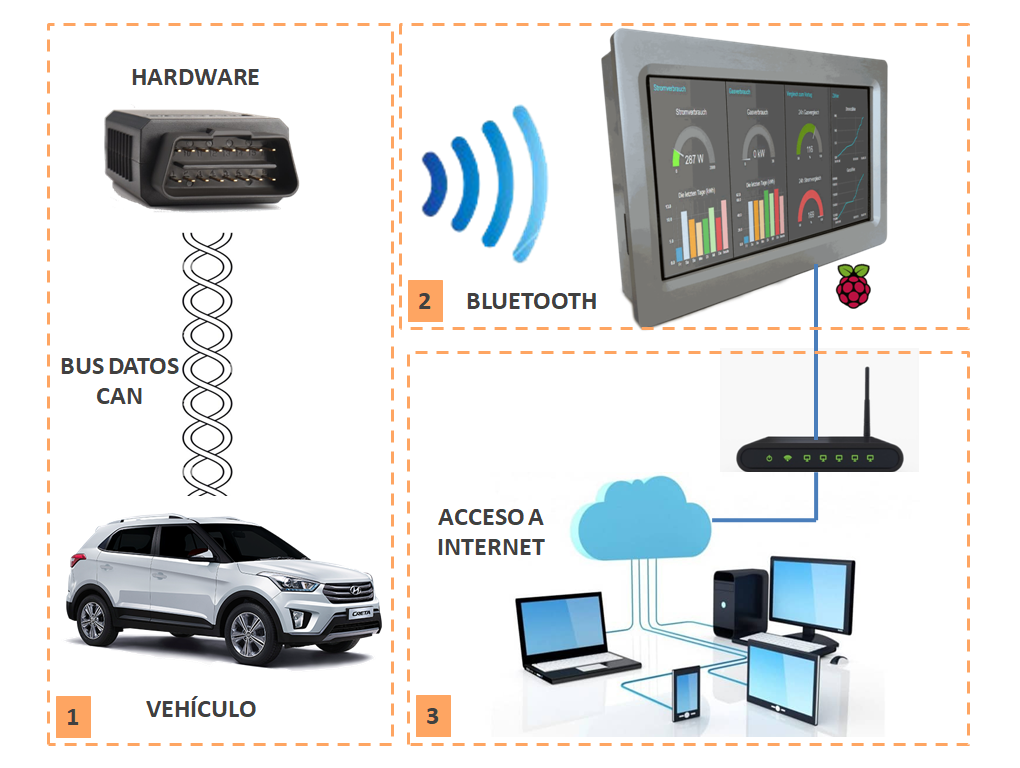
\includegraphics[width=0.9\textwidth]{./Cap00imagen/fig_raspberri_f.png}
	\caption[Sistema CAN con raspberry Pi.]{Sistema CAN con raspberry Pi.\textbf{ Fuente:}  Elaboración Propia.}
	\label{fig_raspberri_c4} % Etiqueta para la referencia.
\end{figure}

% CITAR IMAGEN
%%%%%%%%%%%%%%%%%%%%%%%%%%%%%%%%%%%%%%%%%%%%%%%%%%%%%%%%%%

Para reducir el tamaño físico de hardware CAN se presupuesta usar componentes electrónicos de montajes superficiales y agregar un módulo bluetooth para la conexión con la computadora Raspberry Pi, el presupuesto aproximado de la fabricación completa se logró obtener con la ayuda de la empresa PCBway~\cite{pcbway}, ya que posee unos pasos a seguir para el cálculo de presupuesto para la fabricación completa de un circuito PCB con los componentes incluidos. 
En la Tabla~\ref{tabla:raspberri} se muestran el presupuesto del hardware para este nuevo sistema.
%%%%%%%%%%%%%%%%%%%%% tabla %%%%%%%%%%%%%%%%%%%%%%%%%%%%%%%%
\begin{table}[H]
\begin{center}
\begin{tabular}{ l l r}
\toprule
\textbf{Elementos} & \textbf{Comentario} & \textbf{Costo}  \\ 
\midrule
Hardware CAN    & PCB Fabricado    & 918.000 \\ %\hline
Conector        & OBD II - J1939     & 50.000 \\ %\hline
Módulo          & Bluetooth          & 60.000 \\ %\hline
Computadora     & Raspberry PI 4    & 600.000 \\ %\hline
Pantalla TFT    & 4 pulgadas         & 300.000 \\ %\hline
Protector       & Caja 3D            & 150.000\\ %\hline
\textbf{Total Costos}&  &2 078 000 \\ 
%\hline
\bottomrule


\end{tabular}
\caption{Costo de los elementos para una propuesta mejorada del sistema CAN.}
\label{tabla:raspberri}
\end{center}
\end{table}


Podemos recurrir al software del anterior proyecto y realizar una adaptación del mismo a la Raspberry Pi y modificar el código del microcontrolador para trabajar con el módulo bluetooth, esto agregaría horas de trabajo pero ya no serían tantas si se aprovecha el proyecto original, así en la Tabla~\ref{tabla:extra} se observa los costos de adaptación siguiendo los mismos precios de 30.000/hora-hombre para el trabajo y una cantidad de 240 horas de trabajo distribuida en las distintas partes del proyecto.  

%%%%%%%%%%%%%%%%%%%%% tabla %%%%%%%%%%%%%%%%%%%%%%%%%%%%%%%%
\begin{table}[H]
\begin{center}
\begin{tabular}{l r r r}
\toprule
\textbf{Trabajo Realizado} & \textbf{Horas}&\textbf{Salario por hora Gs.} & \textbf{Importe Gs.} \\ 
\midrule
 Placa Electrónica & 80 & 30 000  & 2.400.000     \\ 
 Software CAN      & 160  & 30.000  & 4.800.000     \\ 
 Diseño de Usuario & 80  & 30.000  & 2.400.000     \\ 
 Programación del Servidor & 80 & 30.000 & 2.400.000 \\ 
  \textbf{Total Costos} &  &  & 12.000.000 \\ \bottomrule
\end{tabular}
\caption{Tabla Costos de mano de obra.}
\label{tabla:extra}
\end{center}
\end{table}
%%%%%%%%%%%%%%%%%%%%%%%%%%%%%%%%%%%%%%%%%%%%%%%%%%%%%%%%%%%%%%%%%%%%



En la \textbf{tabla \ref{tabla:nuevototal}} presentamos el costo total del proyecto teniendo en cuenta los resultados de las tablas anteriores: 

%%%%%%%%%%%%%%%%%%%%% tabla %%%%%%%%%%%%%%%%%%%%%%%%%%%%%%%%
%%%% \textbf{tabla \ref{tabla:hw}} 
\begin{table}[H]
\begin{center}
\begin{tabular}{l r}
\toprule
\textbf{Referencia} & \textbf{Costos}  \\ 
\midrule
Costos Hardware  & 2.078.000     \\ 
Costos Mano de Obra  & 12.000.000     \\ 
Costos Licencias &         0     \\ 
\textbf{Total Costos} & 14.078.000    \\ 
\bottomrule
\end{tabular}
\caption{Tabla costos totales para el nuevo sistema CAN.}
\label{tabla:nuevototal}
\end{center}
\end{table}
%%%%%%%%%%%%%%%%%%%%%%%%%%%%%%%%%%%%%%%%%%%%%%%%%%%%%%%%%%%%%%%%

Rediseñar el sistema aprovechando la primera versión costaría un agregado de 14 078 000 Gs. que es un \textbf{37\%} del costo total del proyecto original. 